\section{Energy Cost, Economics and Demand Response}

\subsection{Economics of Energy}
The demand for energy is a derived demand.
We do not demand energy directly, but rather products and services that require energy.
Even though most things have become more efficient this efficiency increase is often dwarfed by increasing demand.
The prize of energy clearly influences its demand.\\

Some care has to be considered when interpreting energy costs.
Consider mix of energy forms, nominal or real prices, time period and countries.
Recall that energy prices can be very different for different countries.

\subsubsection{The Electricity Price}
One differentiates \textbf{nominal} price (price charged) and \textbf{real} price (adjusted for inflation).
The nominal price of electricity has been steadily increasing, but the real price has been decresing up until the 70s.
Since then the real price has mostly stayed the same.

\subsubsection{The gasoline price}
The nominal gasoline price have increased substantially throughout the last 100 years.
Looking at the real price however it actually shows an overall decrease up until the last 20 years.
Cars have also steadily become somewhat more effective.
The increase of efficiency stopped 1988-2004, which can be explained by low fuel prices.
Figure \ref{fig:car_stats} shows the relationship between fleet size, fuel consumption and \cotwo emissions.

\begin{figure}
    \centering
    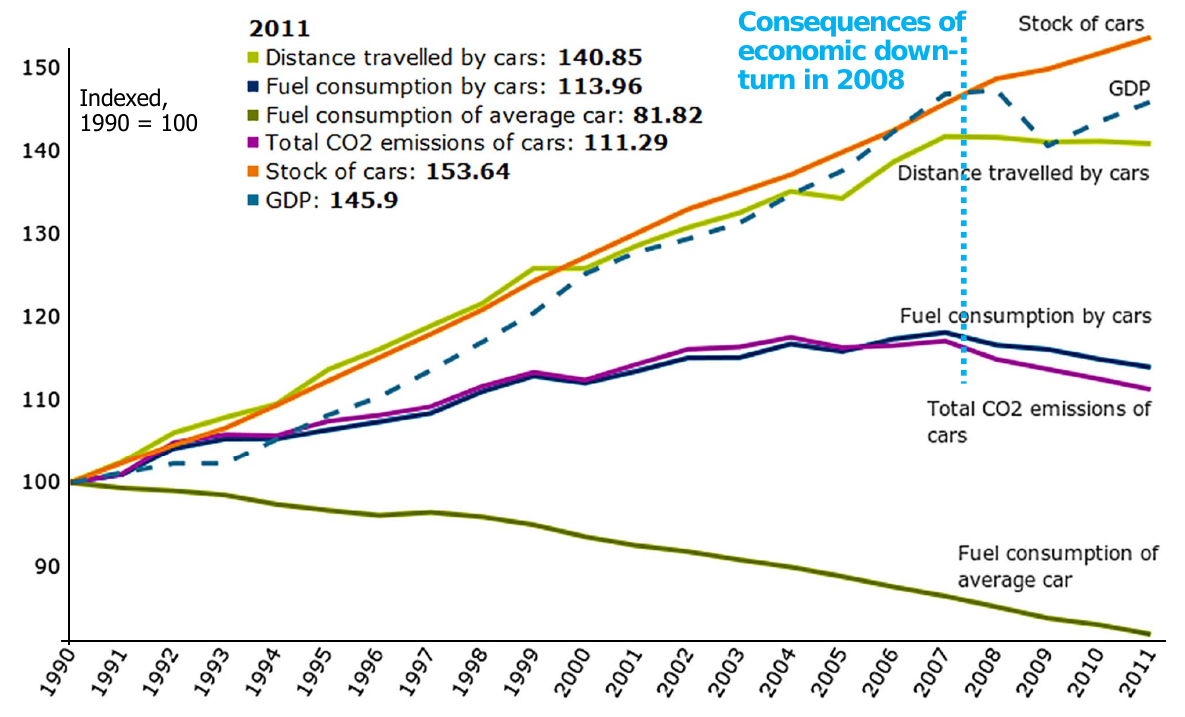
\includegraphics[width=0.85\linewidth]{car_stats}
    \caption{Fuel consumption and \cotwo emissions by cars until 2011}
    \label{fig:car_stats}
\end{figure}

\subsubsection{Household Expenditures}
After the second world war the share of US household income spent on food and energy decreased steadily until 2002.
Lately an increasing share of the household income is spent on energy.
The consumer energy price has been much more volatile than overall consumer prices.
Energy represents $\sim$ 4-5\% of household expenditure.
About half of that (2\%) is electricity.

\subsection{Demand Response (DR)}
The grid requires supply to match demand at all times.
This has traditionally been achieved by letting production follow demand.
Demand response introduces the new paradigm of letting demand follow production.

\subsubsection{Peak loads}
There is a hierarchy of power generating systems that need to cover for the entire demand, see figure \ref{fig:load_curves}.
Peaks in this demand are very expensive.
This is because these peaks require use of special peaker plants.
These plants are typically gas powered and have low utilization rates.
Generally the faster plants can be ramped up the more expensive they are to use.
Switzerland is in a privileged position because of the large amounts of reservoir hydroplants that can be used to cover for the peak loads.\\

\begin{figure}
    \centering
    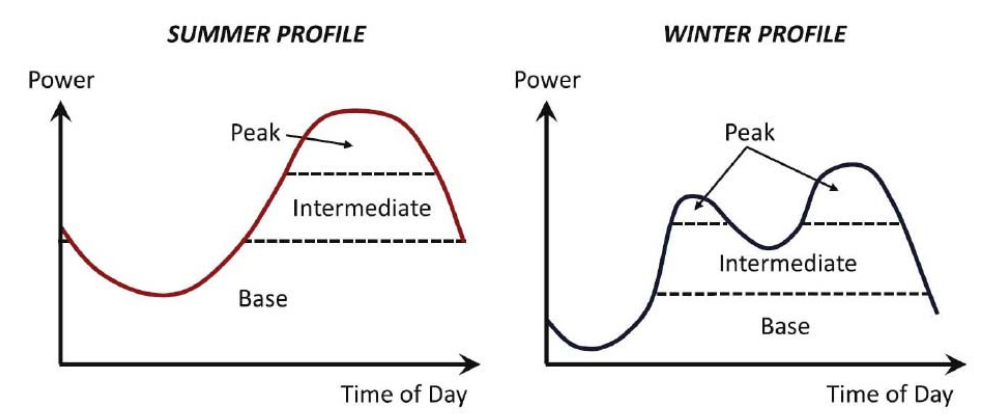
\includegraphics[width=0.7\linewidth]{load_curves}
    \caption{Typical daily load power profiles in the US}
    \label{fig:load_curves}
\end{figure}

The peak demand can be reduced by either load shifting or load shedding, as can be seen in figure \ref{fig:load_shift_shed}.

\begin{figure}
    \centering
    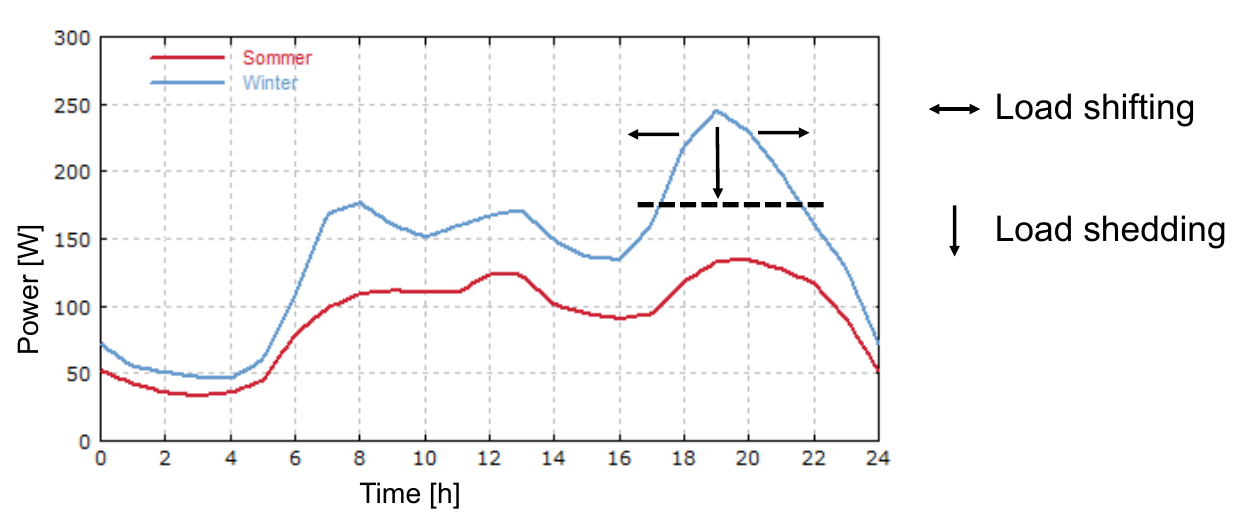
\includegraphics[width=0.8\linewidth]{load_shift_shed}
    \caption{Load shifting and load shedding}
    \label{fig:load_shift_shed}
\end{figure}

\subsubsection{Demand Response for Peak Loads}
Demand response are economical incentives for end-users to change their consumption patterns to reduce peak loads.
Demand response can help in flattening out the load profile and as a response to emergency events.
Demand response can lead to improved grid reliability and lower costs both for utilities and consumers.

\subsubsection{Applying Demand Response}
When a utility company need to decrease the load it send out a demand response signal to any customer being part of a DM program.
The customer then decrease their electricity usage.
These customers have their load measured so that the utility can confirm that the customer does decrease their load.
Customers being part of such a program can be anything from large industrial customers to small residential customers.\\

The special case of demand response for residential customers requires some usefull way of communicating the DM signal.
This can be done through emails, text messages or special hardware.
With integration into home automation system residential DM can also be automated.

\subsubsection{Demand Response Programs}
There are different kinds of demand response programs

\begin{labeling}{}
    \item [\textbf{Time Of Use (TOU)}]
    Fixed rates, not based on current market conditions

    \item [\textbf{Critical Peak Pricing (CPP)}]
    Occasional declaration of a higher price period

    \item [\textbf{Realt Time Pricing (RTP)}]
    Price fluctuates follows market in real time, usually only targeted at industrial customers.

\end{labeling}

Figure \ref{fig:dr_programs} shows the relationship between DM programs, control granularity and telemetry.

\begin{figure}
    \centering
    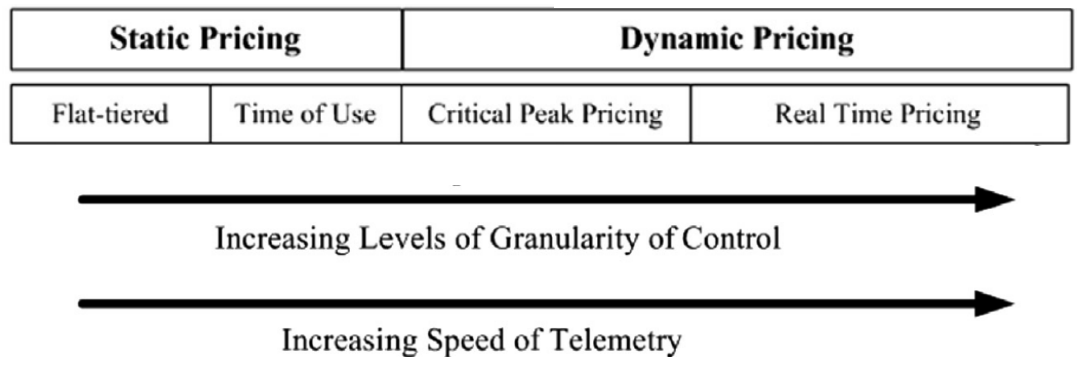
\includegraphics[width=0.7\linewidth]{dr_programs}
    \caption{Demand response programs of increasing control granularity and telemetry speed}
    \label{fig:dr_programs}
\end{figure}

\subsubsection{Consumer Concerns}
Demand response programs face consumer acceptance issues related to
\begin{itemize}
    \item Privacy
    \item External control
    \item Security
    \item Legal issues
\end{itemize}

\subsubsection{Current Use of Demand Response}
In the US demand response is being used to a larger extent than in Europe.
The EU pushes for DR, but there are string regulatory barriers in most countries.
Switzerland is ahead of the EU, starting field trials of residential DR.
